
\section{Introduction}

This chapter presents the theoretical background related to data mining, machine learning, regression methods, ensemble models, and data visualization.
It provides the conceptual foundation needed to understand the implementation choices made later in the report.

\section{Data Mining}

Data Mining is the process of extracting relevant information, patterns, and knowledge from raw data.
It lies at the intersection of statistics, machine learning, and database systems.
Its main objective is not only to describe data but also to reveal hidden structures that can support decision-making.

Typical goals of data mining include classification, regression, clustering, anomaly detection, and association analysis.
In economic contexts, data mining is especially useful for understanding relationships between indicators, discovering structural trends, and building predictive systems.

\section{Machine Learning}

Machine Learning is a branch of artificial intelligence that enables systems to learn from examples rather than relying solely on manually written rules.
A machine learning model uses historical data to identify patterns and generalize them to unseen observations.

\subsection{Supervised Learning}

Supervised learning is based on labeled examples.
The model receives input variables and a target output, then learns a mapping between them.
In this project, supervised learning is used to predict a housing-related target variable from macroeconomic indicators.

Regression and classification are the two main supervised learning settings.
Because our objective is numerical prediction, regression is the most relevant family.

\subsection{Unsupervised Learning}

Unsupervised learning works without labeled targets.
Its objective is to identify internal structures in the data, such as clusters or latent dimensions.
Although this project focuses mainly on supervised prediction, unsupervised ideas remain useful in exploratory analysis.

\section{Regression Models}

Regression models estimate the relationship between one dependent variable and one or several explanatory variables.
They are central tools in both statistics and machine learning.

\subsection{Linear Regression}

Linear regression assumes a linear relationship between the predictors and the response:
\[
y = \beta_0 + \beta_1x_1 + \beta_2x_2 + \dots + \beta_px_p + \varepsilon
\]

Its major strength is interpretability.
However, its performance can degrade when predictors are correlated or when the relationship is not sufficiently linear.

\subsection{Ridge Regression}

Ridge Regression extends linear regression by adding an \(L_2\) penalty on the coefficients:
\[
\min_{\beta} \|y - X\beta\|^2 + \lambda \|\beta\|^2
\]

This regularization reduces overfitting and improves stability in the presence of multicollinearity.
For this reason, Ridge Regression is often used as a solid baseline in predictive tasks involving multiple correlated indicators.

\section{Ensemble Learning and Random Forest}

Ensemble learning combines multiple models in order to obtain a more robust final prediction.
Instead of relying on a single learner, it aggregates several models and often improves performance.

Random Forest is one of the most popular ensemble techniques.
It constructs many decision trees using bootstrap samples and random subsets of features.
The final prediction is obtained by averaging the outputs of all trees.

Its main strengths are:
\begin{itemize}
\item the ability to model non-linear relationships,
\item robustness to noise,
\item resistance to overfitting compared with a single decision tree,
\item and an internal measure of feature importance.
\end{itemize}

For economic datasets where variable interactions can be complex, Random Forest is therefore a strong candidate.

\section{Evaluation Metrics}

Model evaluation is a crucial stage in machine learning.
A model should not only fit the training data but also perform well on unseen observations.
In this project, three standard metrics are used.

\subsection{Mean Absolute Error}

Mean Absolute Error measures the average absolute difference between predicted and observed values:
\[
MAE = \frac{1}{n}\sum_{i=1}^{n} |y_i - \hat{y}_i|
\]

It is easy to interpret and less sensitive to large errors than squared measures.

\subsection{Root Mean Squared Error}

Root Mean Squared Error is defined by:
\[
RMSE = \sqrt{\frac{1}{n}\sum_{i=1}^{n}(y_i - \hat{y}_i)^2}
\]

Because it squares the errors before averaging, it penalizes large deviations more strongly than MAE.

\subsection{Coefficient of Determination}

The coefficient of determination is written as:
\[
R^2 = 1 - \frac{SS_{res}}{SS_{tot}}
\]

It measures the proportion of variance explained by the model.
A value closer to 1 indicates better explanatory power.

\section{Exploratory Data Analysis and Visualization}

Exploratory Data Analysis, often abbreviated as \gls{eda}, is a preliminary stage in which the analyst investigates the dataset through summary statistics and visual representations.
This stage is fundamental because it helps identify missing values, abnormal observations, variable distributions, and potential relationships.

Visualization is not just decorative.
It is a cognitive tool that makes complex patterns easier to understand.
Time series plots, correlation matrices, box plots, and comparative charts allow the analyst to move from raw data to interpretable structure.

\section{Dashboards and Interactive Analytics}

A dashboard is an interface that gathers visual components and filters into a single environment.
In data science projects, dashboards play an important role because they connect technical analysis with practical usability.

In this project, Streamlit was selected as the dashboard framework.
It makes it possible to transform Python code into an interactive web application quickly.
Users can inspect variables, filter data, compare periods, and display predictions without editing the underlying code.

\begin{figure}[H]
\centering
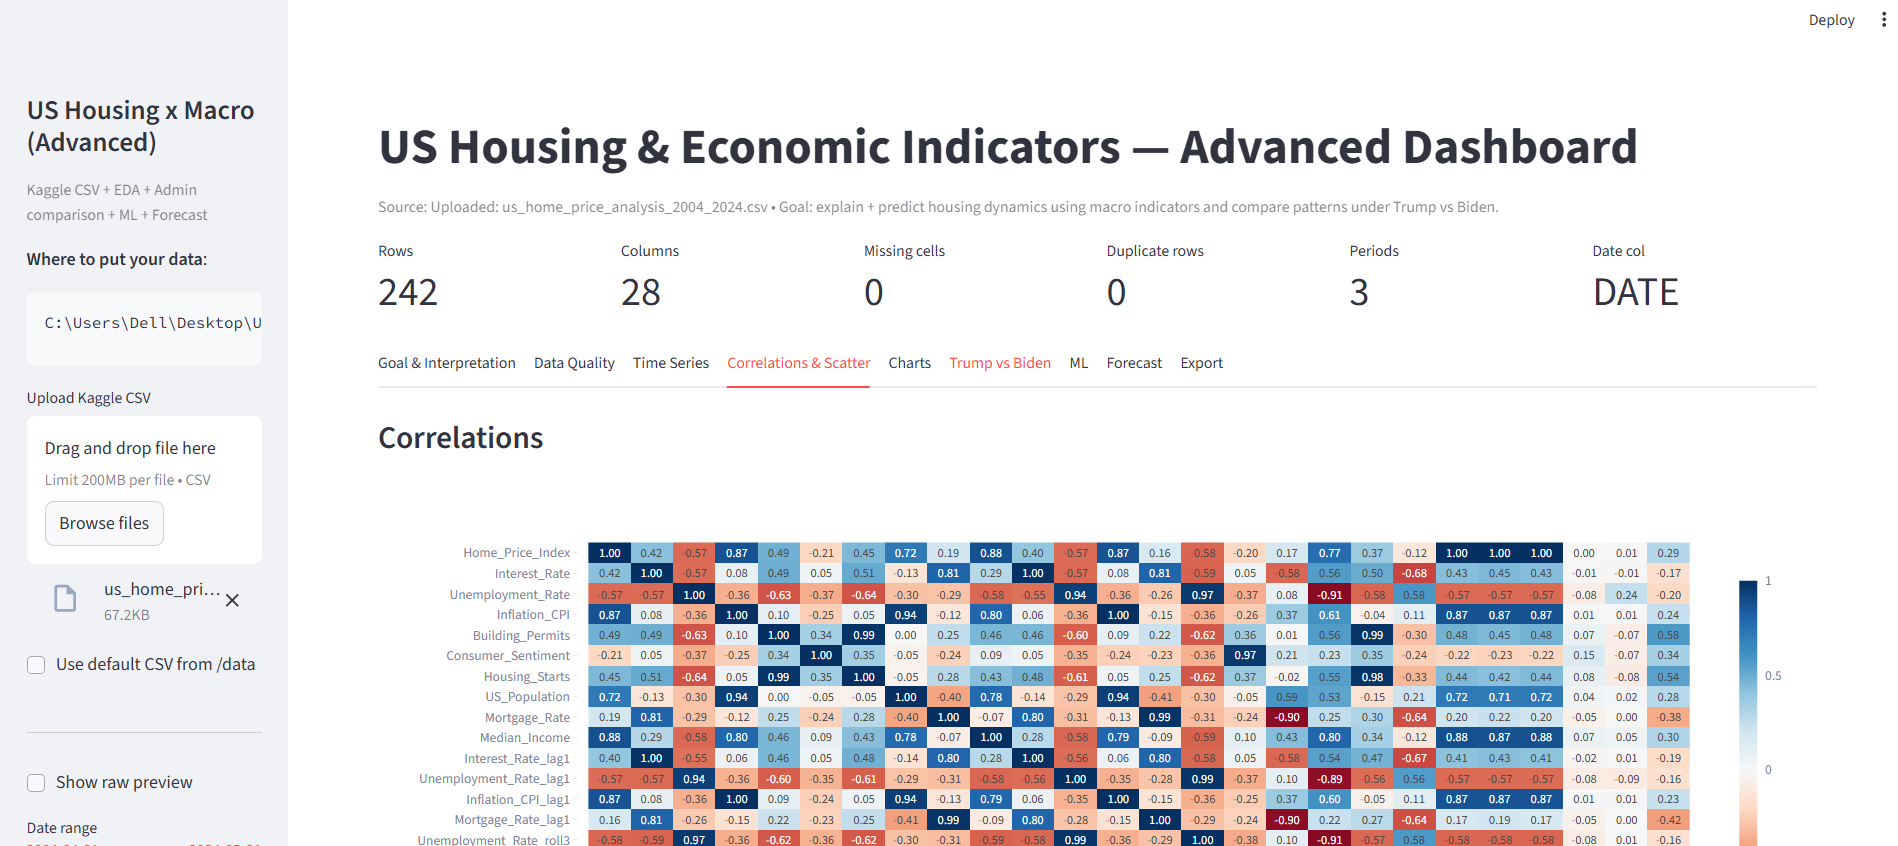
\includegraphics[width=0.82\textwidth]{dashboard_placeholder.png}
\caption{Example placeholder for the dashboard overview. Replace with a real screenshot if available.}
\label{fig:dashboard}
\end{figure}

\section{Applications in Housing Market Analysis}

The housing market has been widely studied using both classical econometric tools and modern machine learning methods.
Researchers and analysts often use explanatory variables such as mortgage rates, income, inflation, and unemployment to understand real estate dynamics.

Machine learning methods are especially useful when the goal is to combine many indicators, uncover non-linear interactions, and build predictive systems that can be refreshed as new data becomes available.
This makes them particularly relevant for dashboards and decision-support tools.

\section{Conclusion}

This chapter reviewed the theoretical concepts underlying the project.
It explained the principles of data mining and machine learning, introduced regression and ensemble methods, and emphasized the role of visualization and dashboards in analytical workflows.
These concepts serve as the basis for the implementation chapter, where the concrete system design and development choices are presented.

\section{OLAP and Multidimensional Analysis}

Online Analytical Processing, usually abbreviated as OLAP, refers to analytical techniques that allow users to examine data across several dimensions. In classical business intelligence, OLAP is used to create summaries such as sales by region, profit by product category, or customer behavior by period. In this project, the same logic is applied to housing and macroeconomic indicators.

The purpose of OLAP in the project is not to replace machine learning. Instead, OLAP complements machine learning by making the data easier to interpret. A predictive model may produce a strong score, but decision-makers often need to understand how averages, medians, changes, and distributions differ across periods or groups.

\subsection{OLAP Operations}

Several OLAP concepts are relevant to the project:
\begin{itemize}
\item \textbf{Roll-up}: aggregation from detailed observations to higher-level summaries, such as monthly values grouped by administration period.
\item \textbf{Drill-down}: movement from an aggregated view to a more detailed view, for example from average housing prices to monthly evolution.
\item \textbf{Slice}: selection of one specific dimension value, such as analyzing only the Biden period.
\item \textbf{Dice}: filtering the data using several dimensions at the same time, such as selecting a period and a set of economic variables.
\item \textbf{Pivot}: rotating dimensions to compare metrics in a table format.
\end{itemize}

\section{AI Chatbots in Data Science Applications}

An AI chatbot is an interface that allows users to interact with a system using natural language. In a data science project, this is useful because many users do not know how to write Python code or interpret model metrics. The chatbot can help explain results, summarize findings, and guide the user toward relevant dashboard pages.

In the project, the chatbot layer is connected to the idea of analytical accessibility. Instead of forcing the user to understand all technical components directly, the system can answer questions such as:
\begin{itemize}
\item What is the strongest driver of housing prices?
\item Which model performed best?
\item What does RMSE mean?
\item Why are lag features useful for forecasting?
\item How should I interpret the OLAP comparison?
\end{itemize}

\section{Prompt Engineering and Prompt Chatbot}

Prompt engineering is the practice of writing clear instructions that guide an AI system toward useful answers. In the context of this project, prompt-based interaction is used to help users formulate analytical questions.

A prompt chatbot differs from a simple chatbot because it can structure the user's request. For example, instead of only answering a vague question, the prompt system can guide the user to specify:
\begin{itemize}
\item the target variable,
\item the period of interest,
\item the model to evaluate,
\item the type of explanation needed,
\item and the business context of the question.
\end{itemize}

This is important because good data analysis depends on good questions. A weak question often produces a weak interpretation, while a precise prompt can lead to a useful analytical answer.

\section{Unsupervised Learning}

Unsupervised learning refers to machine learning methods that do not require labeled output variables. Instead of predicting a known target, these methods search for hidden structure in the data. In housing market analysis, unsupervised learning can help identify similar periods, detect unusual observations, or reduce the dimensionality of the dataset.

\subsection{K-Means Clustering}

K-Means clustering groups observations into a predefined number of clusters. Each cluster contains observations that are similar according to selected numerical features. In this project, K-Means can be used to group months or periods with similar macroeconomic profiles.

\subsection{DBSCAN}

DBSCAN is a density-based clustering method. Unlike K-Means, it does not require all observations to belong to compact spherical clusters. It can also identify noise points. This is useful when the housing market contains abnormal periods, such as crisis months or unusual macroeconomic shocks.

\subsection{Principal Component Analysis}

Principal Component Analysis, or PCA, transforms correlated variables into a smaller set of components. The objective is to reduce dimensionality while preserving as much information as possible. PCA is useful for visualization because complex economic datasets often contain many correlated indicators.

\subsection{Isolation Forest}

Isolation Forest is an anomaly detection method. It isolates observations that are different from the majority of the data. In the housing-market context, anomalies can represent abnormal combinations of prices, interest rates, unemployment, or inflation.

\section{Reinforcement Learning}

Reinforcement learning is a machine learning paradigm in which an agent learns by interacting with an environment. The agent observes a state, chooses an action, receives a reward, and updates its policy. In this project, reinforcement learning is used as an educational module rather than as the main predictive engine.

The main concepts are:
\begin{itemize}
\item \textbf{State}: a representation of the current situation.
\item \textbf{Action}: a decision available to the agent.
\item \textbf{Reward}: feedback that evaluates the quality of the action.
\item \textbf{Policy}: a strategy that maps states to actions.
\end{itemize}

For housing analysis, a simplified example can involve actions such as hold, buy, or wait, depending on whether market indicators suggest upward pressure, affordability stress, or uncertainty. The objective is not to provide financial advice, but to demonstrate how decision policies can be formalized.

\section{Experiment Tracking and Model Registry}

Professional data science requires more than training a single model. Analysts need to know which model was trained, with which features, using which parameters, and with which results. Experiment tracking records these details and supports reproducibility.

A model registry is a structured place where candidate models are stored and compared. It helps identify a champion model, document evaluation results, and prepare for deployment. In the project, these concepts are represented through dashboard modules that track model performance and governance information.

\section{Production Readiness}

Production readiness refers to the checks required before using a data science system in a real environment. A model may perform well in a notebook but still fail in production if the data changes, if missing values appear, or if the model is not monitored.

Important production-readiness checks include:
\begin{itemize}
\item dataset validity,
\item missing-value monitoring,
\item duplicate detection,
\item feature drift,
\item model-card documentation,
\item explainability,
\item and safe interpretation of predictions.
\end{itemize}

This theoretical background supports the implementation described in the next chapter.
